\section{Piano}

\subsection{Brief historical overview}
\bi

\i The modern piano is one of the most popular musical
instruments today.

\i It was invented in 1709 by Bartolomeo Cristofori
in Florence.

\i It is a marvel of engineering, with a very 
sophisticated ``action", which converts the pressing 
of a key into the striking of a hammer against a 
stretched string.

\i The force of the hammer strike is controlled by 
the force with which the key is depressed, 
giving rise to a large dynamic range of the loudness
of the produced sound.

\i The original name of the piano, ``piano-forte", 
literally means ``soft-loud", corresponding to the 
large dynamic range of the produced sound.

\i Precursors of the piano are the {\em clavichord} and 
the {\em harpsichord}, both of which are keyboard
instruments but lack the dynamic range of the modern piano.

\i The strings of a clavichord are struck by a small 
piece of metal (called a {\em tangent}), which is attached 
to the end of each key.
The tangent stays in contact with the struck string,
which vibrates between the location of the tangent and 
the bridge.

\i The strings of a harpsichord are plucked by a
a {\em plectrum} (originally made from a birds quill),
which is attached to a vertical piece of wood 
(called a {\em jack}) at the end of each key.
Since the force of the plucking is {\em independent} 
of the force used to depress the key, the loudness
of a note produced on a harpsichord is fixed---i.e.,
it cannot be changed like a piano.

\ei
%%%%%%%%%%%%%%%%%%%%%%%%%%%%%%
\subsection{Construction of a grand piano}
\bi

\i The main parts of a modern grand piano are the
keyboard, action, strings, soundboard and frame.

\i Figure~\ref{f:grand-piano-exploded} is an 
exploded view of a grand piano, and 
Figure~\ref{f:piano-action1} shows a
simplified view of a cross-section of the piano.
%
\begin{figure}[htbp]
\begin{center}
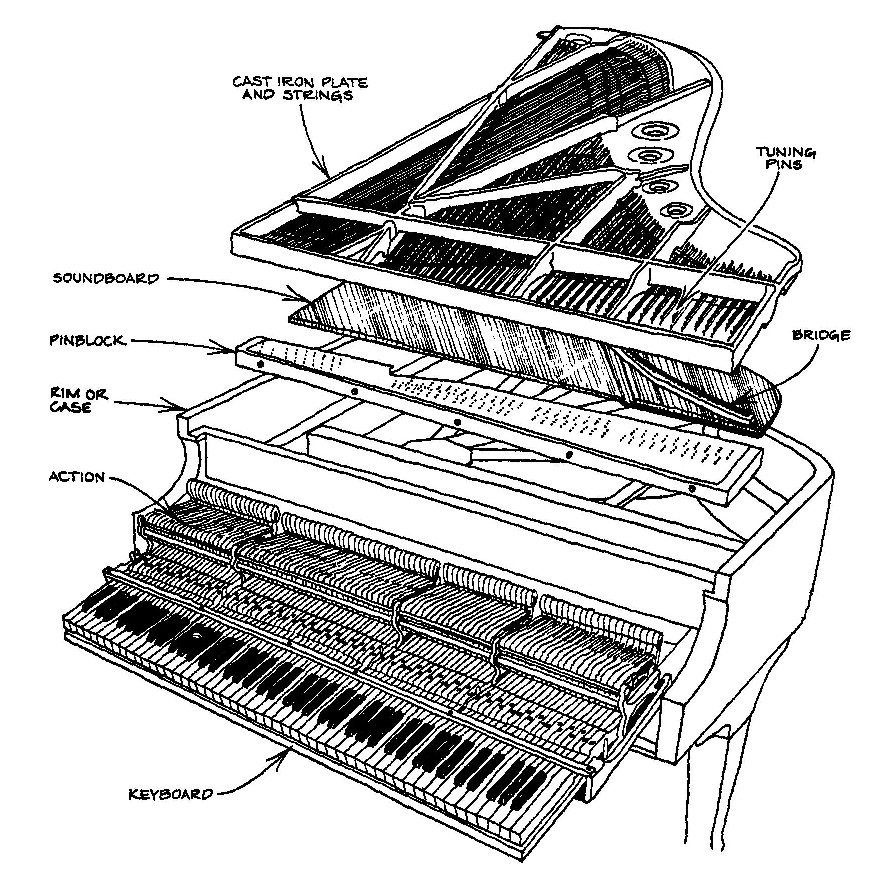
\includegraphics[width=\textwidth]{grand-piano-exploded.jpg}
\caption{
Exploded view of a grand piano.
(Figure taken from 
{\tt http://www.motspheres.com}.)}
\label{f:grand-piano-exploded}
\end{center}
\end{figure}
%
\begin{figure}[htbp]
\begin{center}
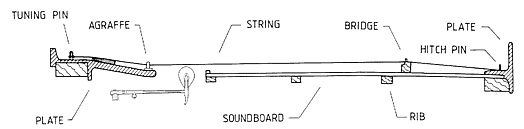
\includegraphics[width=.9\textwidth]{piano-action1.jpg}
\caption{
Simplified cross-section of a grand piano, showing a hammer, 
a string, and its connection to the soundboard and frame via
the bridge and pins.
(Figure taken from 
{\tt http://www.speech.kth.se/music/}.)}
\label{f:piano-action1}
\end{center}
\end{figure}

\i There are 88~keys corresponding to the notes
A${}_0$ to C${}_8$, tuned to equal-temperament
(but see details in a later section).

\i There are 243 strings, varying in length 
from 2~m at the bass end to 5~cm at the treble end.

- 8 single strings, wrapped (lowest notes)

- 5 pairs of strings, wrapped

- 7 triples of strings, wrapped

- 68 triples of strings, unwrapped (highest notes)

\i Wrapping increases the mass density of the string
needed for the bass notes, without increasing
the {\em inharmonicity} of the strings too much.
(The inharmonicity of the strings is due to the 
inherent stiffness of the wire used for piano strings.  
See below for more details.)

\i The individual strings are typically subject to
tensions of order 1000~N (or about 220~lb).
Since there are over 200 piano strings, this means
that the piano must support over 40000~lb (or 20 tons)
of tension.

\i A cast iron frame is needed to support such large
forces.

\i The soundboard is generally made of spruce, 
approximately 1~cm thick.
The vibrating strings are coupled to the soundboard
via the bridge.
The soundboard is what produces the large volume of
sound produced by a piano.

\i Figure~\ref{f:piano-action2} shows a detailed view of
the piano ``action", which converts the pressing of a key
into the striking of a hammer against a piano string.
%
\begin{figure}[htbp]
\begin{center}
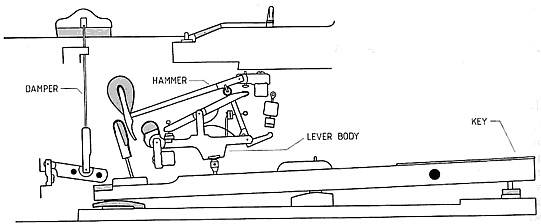
\includegraphics[width=.9\textwidth]{piano-action2.jpg}
\caption{
Detailed view of the piano action, which connects a key 
to its hammer.
(Figure taken from 
{\tt http://www.speech.kth.se/music/}.)}
\label{f:piano-action2}
\end{center}
\end{figure}

\i \demo Watch the YouTube video ``Grand Piano Action Model"\\
({\tt https://www.youtube.com/watch?v=95hnnb7KLAg}) to see
a piano action in action.

\ei
%%%%%%%%%%%%%%%%%%%%%%%%%%%%%%%%%%%%%%%%%%%%%%%%%%%%%%%%%%%%%
\subsection{Attack and decay transients of piano notes} 
\bi

\i The notes produced by a piano have a very short attack 
transient and a long decay transient.

\i The decay transient actually has two phases:
a period of rapid decay followed by a period of a 
slower decay, sometimes called the {\em aftersound}.

\i The different decay rates are due to slight mistunings 
(on purpose) of the three strings per note.
The tensions in the neighboring strings are adjusted so that
the corresponding frequencies differ by about 1 or 2 cents.

\i When a note is played, the three strings initially vibrate
in phase and efficiently transfer their energy to the soundboard,
each pulling on the bridge in the same direction at the same time.
This leads to a loud sound with a rapid decay.

\i But as time progresses, the strings begin to vibrate 
{\em out of phase} with one another, leading to less efficient 
transfer of energy to the soundboard, since the vibrations
pull on the bridge in opposite directions at the same time.
This leads to a softer sound with a slower decay.

\i \demo
Play the matlab file {\tt pianoC4.mat}
both forward and backward using the routine 
{\tt playrecordedsound.m} to illustrate the 
difference between the attack and decay transients.

\i \demo
Do the same with {\tt happybirthday-backwards.mat}.

\i A musician can use the {\em pedals} on a piano to 
change how the notes sound.

- Right pedal: sustain pedal; lifts the dampers so that
all notes are sustained 

- Left pedal: expression pedal (or {\em una corda} pedal); 
shifts the action slightly so that the hammers strike only 
2 of the 3 strings

- Center pedal: ({\em sostenuto} pedal); 
sustains only those notes that were depressed {\em prior} 
to depressing the pedal, and not the subsequent notes

\ei
%%%%%%%%%%%%%%%%%%%%%%%%%%%%%%%
\subsection{Inharmonicity of piano strings}
\bi

\i Due to the inherent stiffness of a real piano wire, 
the frequencies of the vibrational modes are not exact 
harmonics of the fundamental frequency.

\i There is a bending force intrinsic to the wire, in addition
to the applied tension, which tends to increase the frequency
of the vibrational modes.

\i The frequencies of the vibrational modes are given by
%
\be
f_n 
%= nf_0\,\sqrt{1+Bn^2} 
=nf_0\left(1+\frac{1}{2}n^2 B\right)
\ee
%
where
%
\be
f_0 = \frac{1}{2L}\sqrt{\frac{\tau}{\mu}}\,,
\qquad
B = \frac{\pi^3 r^4 E \mu f_0^2}{\tau^2}
= \frac{\pi^3 r^4 E}{4 L^2 \tau}
\ee
%

\i In the above formulae, $f_0$ is the frequency that an
ideal string would have,
$E$ is Young's modulus (which specifies the stiffness
of the material), $\tau$ is the tension in the string,
$r$ is its radius, $L$ is its length, and $\mu$ is its 
linear mass-density (mass/length).
The formula for $f_n$ assumes that $n^2 B\ll 1$, 
which is typically the case.

\i Note that the fundamental frequency $f_1$ for a real
string is not the same as $f_0$ for an ideal string, 
but equals
%
\be
f_1 = f_0\left(1+\frac{1}{2}B\right)
\quad
{\rm which\ implies}
\quad
f_n 
=nf_1\left[1+\frac{1}{2}(n^2-1)B\right]
\ee
%
for the vibrational frequencies in terms of the
fundamental frequency $f_1$ for the real string.

\i The deviation of these frequencies from 
pure harmonics is proportional to $(n^2-1)$.
For small values of $n$ the difference of $f_n$ from
its pure harmonic $nf_1$ is small, but as 
$n$ increases the difference can become large.

\i \ex
For a steel piano string which has 
$E=2\times 10^{11}~{\rm N/m}^2$, 
$\rho = 7840~{\rm kg/m}^3$, 
$r=0.5~{\rm mm}$, 
$\tau = 150~{\rm lb}$, and a length $L$ corresponding
to the fundamental frequency $f_0= 231.63~{\rm Hz}$ 
(C${}_4$) for an ideal string:
%
\be
\frac{f_2}{2 f_1} = 1~{\rm cent}\,,
\quad
\frac{f_3}{3 f_1} = 3~{\rm cent}\,,
\quad
\frac{f_4}{4 f_1} = 5~{\rm cent}\,,
\quad
\frac{f_8}{8 f_1} = 20~{\rm cent}\,,
\quad
\frac{f_{16}}{16 f_1} = 79~{\rm cent}
\ee
%
so the deviations for the second, third, and fourth
octaves are definitely noticeable.

\i The deviation is smaller if one uses {\em wrapped}
strings, which are more flexible than solid strings
with the same mass density.
This reduces the deviation to about 30~cents for the
fourth octave instead of 79~cent, as calculated above
for solid steel wire strings.

\i As we shall see in the next subsection, pianos are 
actually tuned to have {\em stretched} octaves corresponding
to these higher frequency ratios, as first 
systematically studied by O.L.~Railsback around 1960.

\ei
%%%%%%%%%%%%%%%%%%%%%%%%%%%%%%%%%
\subsection{Stretched tuning}
\bi

\i A piano is tuned to equal temperament within an
octave, and has stretched tuning (due to the inharmonicity
of the strings) from one octave to another.

\i Stretched tuning means that the higher octaves are 
tuned sharp and lower octaves tuned flat relative
to equal-tempered tuning, as we shall see below.

\i The chromatic notes in a octave are equally spaced
by a semitone interval, which corresponds to the frequency
ratio $2^{1/12} = 1.0596$.

\i \underline{Step 1}: 
The piano tuner uses a tuning fork 
(or an electronic tuning device) to set one note in the 
octave, e.g., C${}_4$, to its correct equal-tempered
value.
In this case, C${}_4$ should have the absolute frequency 261.63~Hz.

\i \underline{Step 2}: 
The tuner then ``lays the temperament" by tuning all of 
the chromatic notes in an octave interval (e.g., C${}_4$ to 
C${}_5$) by working around the circle of
fifths: C to G, G to D, etc.

\i Since the frequency ratio of an equal-tempered fifth
%
\be
2^{7/12} = 1.4983
\ee
%
is less than that of a perfect fifth ($3/2=1.5$), there
will be beats between the second harmonic of G${}_4$ and
the 3rd harmonic of C${}_4$.

\i The frequency difference 
between an equal-tempered fifth and a perfect fifth 
is given by
%
\be
\delta = 1.4983f_1 - 1.5f_1 = -0.0017 f_1
\ee
and the corresponding beat frequency is
%
\be
f_{\rm beat} = 2|\delta|= 0.0034 f_1
\ee

\i Since the beat frequency depends on $f_1$, it will be
different when tuning the equal-tempered fifths 
G${}_4$ to D${}_5$, D${}_4$ to A${}_4$, etc., than it 
is for tuning the equal-tempered fifth C${}_4$ to G${}_4$.

\i Table~\ref{t:beatfreqsET} lists the beat frequencies 
for equal-tempered tuning of the chromatic scale from 
C${}_4$ to C${}_5$ using the above method of fifths.
%
\begin{table}[htbp]
\begin{center}
\begin{tabular}{|l|c|c|}
\hline
Interval & ET freq of first note (Hz) & Beat frequency (Hz) \\
\hline
C${}_4$ to G${}_4$ & 261.63 & 0.89 \\
G${}_4$ to D${}_5$ & 392.00 & 1.33 \\
D${}_4$ to A${}_4$ & 293.66 & 1.00 \\
A${}_4$ to E${}_5$ & 440.00 & 1.50 \\
E${}_4$ to B${}_4$ & 329.63 & 1.12 \\
B${}_3$ to F${}^\sharp_4$ & 246.94 & 0.84 \\
F${}^\sharp_4$ to C${}^\sharp_5$ & 369.99 & 1.26 \\
C${}^\sharp_4$ to G${}^\sharp_4$ & 277.18 & 0.94 \\
G${}^\sharp_4$ to D${}^\sharp_5$ & 415.30 & 1.41 \\
D${}^\sharp_4$ to A${}^\sharp_4$ & 311.12 & 1.06 \\
A${}^\sharp_4$ to F${}_5$ & 466.16 & 1.58 \\
F${}_4$ to C${}_5$ & 349.23 & 1.19 \\
\hline
\end{tabular}
\caption{Frequencies and beat frequencies 
for equal-tempered tuning of the chromatic scale from 
C${}_4$ to C${}_5$ using the method of fifths.
(After a similar table in ``Science of Sound," by
Rossing, Moore, and Wheeler.)}
\label{t:beatfreqsET}
\end{center}
\end{table}

\i \underline{Step 3}:
The piano tuner listens for these beat frequencies,
adjusting the tension in the G${}_4$ string, 
D${}_5$ string, etc.\ 
to give the beat frequencies in this table.

\i NOTE: Rather than try
to listen for e.g., 0.89 beats per second, the tuner 
listens for 8.9 beats in a 10 second interval.
The counting of beats is easier to do over this longer 
time interval.

\i \underline{Step 4}:
Once the chromatic notes in an octave have been
set, the piano tuner moves from that octave to other
octaves by matching e.g., the second harmonic of G${}_4$ 
with the fundamental of G${}_5$, etc., and 
then the fourth harmonic of C${}_4$ with the 
fundamental of C${}_6$, etc.
(This is done by adjusting the tension of the G${}_5$ 
string to eliminate any beats with the second harmonic 
of G${}_4$, etc.)

\i But since the second harmonic of any note has 
a frequency that is greater than $2\times$ its
fundamental frequency (due to the inharmonicity of
the piano strings), the frequency of the new note
will be {\em sharper} than the 
equal-tempered frequency for that new note.

\i And as one tunes the higher octaves the notes
become even sharper, since the deviation of the
frequencies from true harmonics
increases with $n$ as we saw above.

\i Using similar reasoning, one can show that for 
octaves below C${}_4$ (e.g., starting with 
C${}_3$, C${}_2$, etc.), 
the notes will be tuned {\em flatter} than
equal-tempered tuning.

\i Around 1960 O.L. Railsback measured the tunings 
of many pianos.
Figure~\ref{f:Railsback}, called a Railsback
curve, shows the deviation of the frequencies of 
the notes of an actual piano (in green) from that 
of equal-tempered tuning (which corresponds to 
a horizontal line at 0 cents).
The jagged line is an average of tunings measured
from several pianos.
%
\begin{figure}[!htbp]
\begin{center}
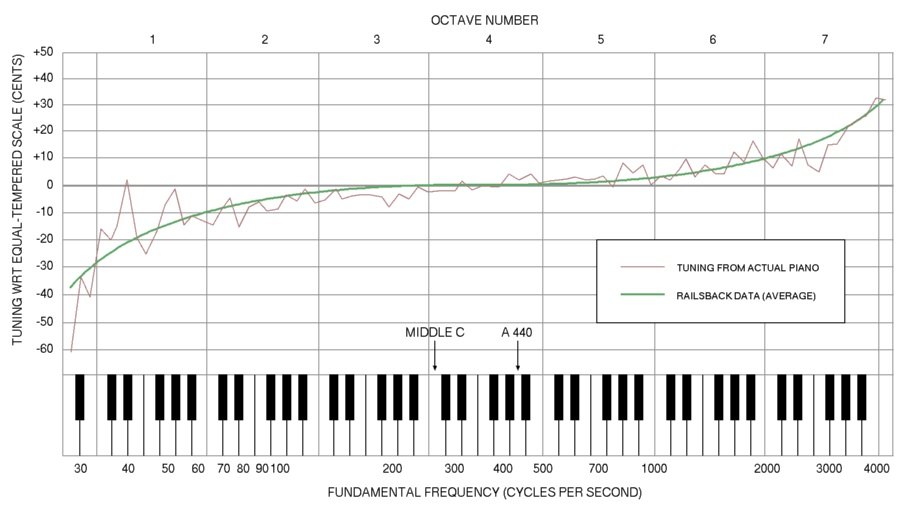
\includegraphics[width=\textwidth]{Railsback.jpg}
\caption{A Railsback curve showing the 
deviation of the frequencies of the notes of 
a single piano (and an average for many piano)
from that of equal-tempered tuning.
(Figure taken from 
{\tt http://en.wikipedia.org}.)}
\label{f:Railsback}
\end{center}
\end{figure}
%
\FloatBarrier

\i This sloping curve, which indicates flatter notes
in the lower octaves and sharper notes in the upper
octaves, is an illustration of stretched tuning.

\ei

